\documentclass[12pt]{article}
\usepackage[margin=2.5cm]{geometry}
\usepackage{enumerate}
\usepackage{amsfonts}
\usepackage{amsmath}
\usepackage{fancyhdr}
\usepackage{amsmath}
\usepackage{amssymb}
\usepackage{amsthm}
\usepackage{mdframed}
\usepackage{graphicx}
\usepackage{subcaption}
\usepackage{adjustbox}
\usepackage{listings}
\usepackage{xcolor}
\usepackage{booktabs}
\usepackage[utf]{kotex}

\definecolor{codegreen}{rgb}{0,0.6,0}
\definecolor{codegray}{rgb}{0.5,0.5,0.5}
\definecolor{codepurple}{rgb}{0.58,0,0.82}
\definecolor{backcolour}{rgb}{0.95,0.95,0.92}

\lstdefinestyle{mystyle}{
    backgroundcolor=\color{backcolour},
    commentstyle=\color{codegreen},
    keywordstyle=\color{magenta},
    numberstyle=\tiny\color{codegray},
    stringstyle=\color{codepurple},
    basicstyle=\ttfamily\footnotesize,
    breakatwhitespace=false,
    breaklines=true,
    captionpos=b,
    keepspaces=true,
    numbers=left,
    numbersep=5pt,
    showspaces=false,
    showstringspaces=false,
    showtabs=false,
    tabsize=1
}

\lstset{style=mystyle}

\begin{document}
\title{CSC148 Worksheet 17 Solution}
\author{Hyungmo Gu}
\maketitle

\section*{Question 1}
\begin{itemize}
    \item

    We need to implement the base case for this function.

    \bigskip

    The docstring tells us the function does nothing if \textless obj \textgreater is an int.

    \bigskip

    Using this fact, we can write that

    \bigskip

    \begin{lstlisting}[language=python,caption={worksheet\_17\_q1\_solution.py}]
    def add_one(obj: Union[int, List]) -> None:
        """Add one to every number stored in <obj>. Do nothing if <obj> is an int.
        If <obj> is a list, *mutate* it to change the numbers stored.
        >>> lst0 = 1
        >>> add_one(lst0)
        >>> lst0
        1
        >>> lst1 = []
        >>> add_one(lst1)
        >>> lst1
        []
        >>> lst2 = [1, [2, 3], [[[5]]]]
        >>> add_one(lst2)
        >>> lst2
        [2, [3, 4], [[[6]]]]
        """

        if isinstance(obj, int):
            return obj
    \end{lstlisting}

    \bigskip

    \begin{mdframed}
        \underline{\textbf{Correct Solution:}}

        \bigskip

        We need to implement the base case for this function.

        \bigskip

        The docstring tells us the function does nothing if \textless obj \textgreater is an int.

        \bigskip

        Using this fact, we can write that

        \bigskip

        \begin{lstlisting}[language=python,caption={worksheet\_17\_q1\_solution.py}]
        from typing import Union, List, Optional

        def add_one(obj: Union[int, List]) -> None:
            """Add one to every number stored in <obj>. Do nothing if <obj> is an int.
            If <obj> is a list, *mutate* it to change the numbers stored.
            >>> lst0 = 1
            >>> add_one(lst0)
            >>> lst0
            1
            >>> lst1 = []
            >>> add_one(lst1)
            >>> lst1
            []
            >>> lst2 = [1, [2, 3], [[[5]]]]
            >>> add_one(lst2)
            >>> lst2
            [2, [3, 4], [[[6]]]]
            """

            if isinstance(obj, int):
        # =========== Correction ===========
                pass

        if __name__ =='__main__':
            import doctest
            doctest.testmod()
        # ==================================
        \end{lstlisting}
    \end{mdframed}
\end{itemize}

\section*{Question 2}
\begin{itemize}
    \item No values in \textit{obj} would change.

    \begin{center}
    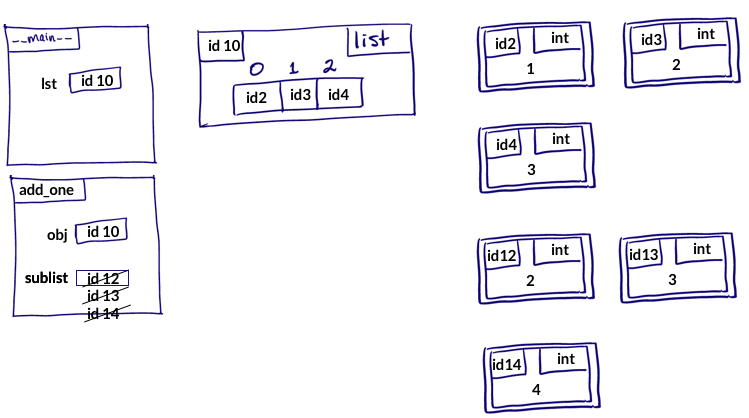
\includegraphics[width=0.8 \linewidth]{images/worksheet_17_q2_solution.png}
    \end{center}
\end{itemize}

\section*{Question 3}
\begin{lstlisting}[language=python,caption={worksheet\_17\_q3\_solution.py}]
    from typing import Union, List, Optional

    def add_one(obj: Union[int, List]) -> None:
        """Add one to every number stored in <obj>. Do nothing if <obj> is an int.
        If <obj> is a list, *mutate* it to change the numbers stored.
        >>> lst0 = 1
        >>> add_one(lst0)
        >>> lst0
        1
        >>> lst1 = []
        >>> add_one(lst1)
        >>> lst1
        []
        >>> lst2 = [1, [2, 3], [[[5]]]]
        >>> add_one(lst2)
        >>> lst2
        [2, [3, 4], [[[6]]]]
        """

        if isinstance(obj, int):
            pass
        else:
            for i in range(len(obj)):
                if isinstance(obj[i], int):
                    obj[i] += 1
                else:
                    add_one(obj[i])


    if __name__ =='__main__':
        import doctest
        doctest.testmod()
\end{lstlisting}


\end{document}